\section{Uczenie nadzorowane}

Drugie podejście do uczenia bazuje na implementacji rozwiązania opartego na uczeniu nadzorowanym.

Podczas działania modułu trenującego rozgrywane są gry, z losowym początkowym ustawieniem planszy. Dla każdej sekwencji par stan - akcja, przypisywana była nagroda, zgodna z wynikiem gry dla rozpatrywanego gracza.

Przykładowo:

$$\big((s_{1}, a_{1}), (s_{2}, a_{2}), (s_{3}, a_{3})\big) \rightarrow 1$$

Następnie każdy z ruchów dodawany jest do słownika, gdzie każda z krotek jest kluczem, natomiast ich wartościami są krotki, zbudowane według następującego schematu.

$$(X_{win}, O_{win}, Draw)$$

Tak otrzymane krotki wartości przekształcane są tak, że $\frac{x_{wins} - o_{wins} - 0.25 draws}{total\_games}$, aby każda z nich została przekształcona na pojedynczą wartość ze zbioru $\{-1, 1\}$.

Dane, które zostały ostatecznie otrzymane, wykorzystane są do nauczania sieci neuronowej, która dla każdego stanu daje odpowiedź,czy ruch jest odpowiedni, czy nie.

Architektura sieci jaką wykorzystano:
\begin{itemize}
	\item 36 neuronów w warstwie wejściowej (aktywacja ReLu);
	\item 18 neuronów w warstwie ukrytej (również aktywacja ReLU);
	\item 1 neuron wyjściowy (aktywacja $tanh$).
\end{itemize}

\begin{figure}[H]
	\centering
	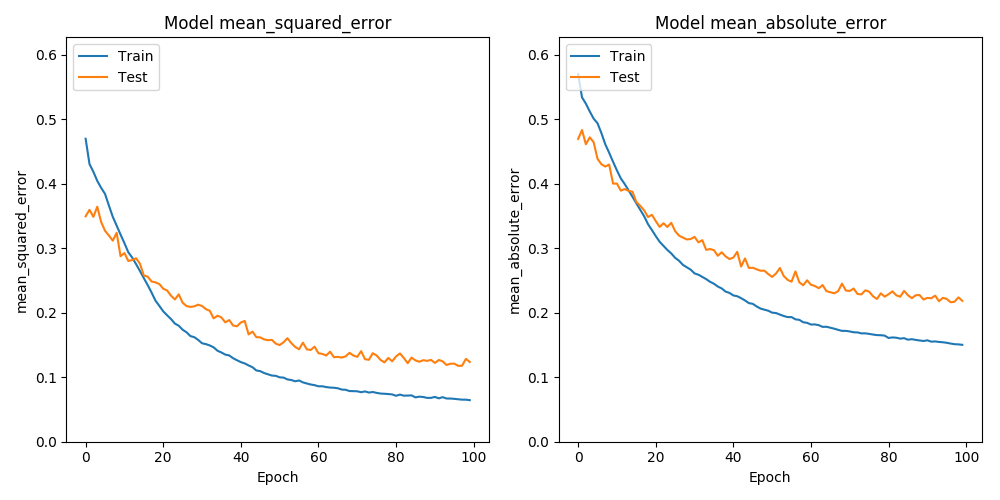
\includegraphics[width=0.7\linewidth]{imgs/nn_plots}
	\caption{Krzywa uczenia.}
\end{figure}

\pagebreak